\documentclass[a4paper]{article}
\usepackage[utf8]{inputenc}
\usepackage[spanish]{babel} 
\renewcommand{\spanishtablename}{Tabla} 
\spanishdecimal{.}
\usepackage{verbatim}
\usepackage{amssymb}
\usepackage{multirow}
\usepackage{subcaption}
\usepackage{wrapfig}
\usepackage{graphicx}
\usepackage{hyperref}
\usepackage{mathtools}
\usepackage{float}
\usepackage{siunitx}
\renewcommand{\thefootnote}{\arabic{fotnote}}
\setlength{\parskip}{\baselineskip} 
\usepackage{pdfpages}

\begin{document}

\begin{titlepage}
\paragraph{}

\begin{center}
\vspace*{0.10in}
\begin{figure}
\raggedleft

\includegraphics[scale=0.12]{unam.png}
\hspace{7.2cm}
\raggedright

\includegraphics[scale=0.15]{fac.png}    
\end{figure}
\vspace*{0.5in}
UNIVERSIDAD NACIONAL AUTÓNOMA DE MÉXICO\\
\vspace*{0.2in}
FACULTAD DE CIENCIAS \\
\vspace*{0.5in}
\begin{large}
Laboratorio de Calor, Ondas y Fluidos\\
\end{large}
\vspace*{0.2in}
\begin{Large}
\textbf{Práctica 3} \\
\textbf{Calor Específico} \\
\end{Large}
\vspace*{0.3in}
\vspace*{0.3in}
\rule{80mm}{0.1mm}\\
\vspace*{0.1in}
\begin{large}
Profesor:  Quintanar Robles, Luis  \\
Ayudante: Quintanar Cortés, Luis Enrique \\
Mesa 1\\
Fecha de la práctica: 3 de septiembre de 2019.\\
Alumnos: León Arenal Sebastian.\\
Robledo Ibarra Emiliano. \\
Toledo Castañeda, Akim Tarik.\\

\end{large}
\end{center}
\end{titlepage}



\section*{Resumen.}
Se calculó el calor específico de tres objetos distintos por medio de un calorímetro cuantificando la masas que actuaron y sus temperaturas al inicio del fenómeno y al equilibrio. Se nombraron los tres objetos por su color: plateado ($C_e = 0.27 \pm 0.03 \frac{cal}{gr{\circ}C}$), dorado ($C_e = 0.113 \pm 0.014 \frac{cal}{gr{\circ}C}$) y cobrizo ($C_e = 0.10 \pm 0.09 \frac{cal}{gr{\circ}C}$). Mediante una aproximación se encontraron algunos candidatos para los materiales que constituyen los objetos medidos, por su calor específico el plata es cercano al aluminio, el dorado al latón o acero, pero el tercero resulta más difícil debido a su incertidumbre por lo que resultó inconcluso dicho calor específico. Se concluyó que es necesario mejorar el método de obtención de la temperatura del objeto aprovechando propiedades como el equilibrio térmico.

\section*{Introducción.}
La Termodinámica estudia la interacción entre el calor y otras manifestaciones de energía; gracias a esta rama de la física nos ha sido posible construir modelos cuyo papel es  fundamental para diversas áreas. El equilibrio térmico es un concepto fundamental para la termodinámica. Éste habla de un estado en el cual la energía de dos o más sistemas en contacto llegan a igualarse de manera que la energía característica en ambos sistemas sea homogénea (como si se tratase de un solo sistema). Usualmente se habla del calor y la temperatura como iguales pero no es así aunque están estrechamente relacionadas. Pues el calor es la energía que se transfiere de cuerpo a otro, la temperatura es la medida que expresa el grado o nivel de calor de los cuerpos o del ambiente.

Mediante observación y experimentación, se puede notar que determinados objetos aumentan más rápido su temperatura a comparación de otros, un ejemplo de esto es cuando se usa una olla de metal para calentar agua  en la estufa, es posible notar cierta diferencia puesto que el metal requiere menor exposición al fuego para elevar su temperatura. 

Este resultado arroja una hipótesis: \textit{Distintos materiales expuestos a la misma fuente de calor, requieren de más o menos tiempo para elevar su temperatura}; se sabe que los materiales absorben de manera distinta el calor y este flujo de calor es proporcional a la masa y su variación en la temperatura. Dada la hipótesis anterior, en esta práctica se buscó experimentalmente la constante (normalmente llamada \textit{calor específico}) que cumpla dicha relación mediante el uso de un calorímetro, un termómetro y una balanza. Se buscó una ecuación tal que considere las temperaturas de los objetos y su masa, la ecuación que expresa estas medidas es la que habla del calor que absorbe y transfieren los objetos, la suma entre ambas cantidades en un sistema cerrado son contrarias y su suma es igual a cero, es decir $\Delta Q_{abs} + \Delta Q_{trans} = 0$.

Para analizar este fenómeno se usó como hipótesis la Ley Cero de la Termodinámica que propone lo siguiente: \textit{Si dos sistemas están en equilibrio térmico independientemente con un tercer sistema, deben estar en equilibrio térmico entre sí}. Mediante esta ley se puede medir la diferencia de temperaturas que es parte esencial de la cuantificación del calor suministrado, además de ello se supuso que el sistema donde ambos sistemas entran en contacto está aislado (de forma que no hubo una pérdida de energía). 


\section*{Procedimiento.}
Se llenó un vaso de precipitado de 500mL con agua y dentro se colocó el  objeto metálico. Con una parrilla eléctrica se calentó dicho sistema. Cuando el agua comenzó a hervir se retiró el objeto metálico del interior del vaso con la ayuda de unas pinzas. Al retirar el objeto del vaso se debe tener mucho cuidado; si las pinzas no sujetan con suficiente fuerza el objeto, éste puede resbalar y, en el peor de los casos, romper el vaso de precipitados.También se debe tener cuidado de no derramar agua sobre la parrilla al momento de retirar el objeto. Una vez que el objeto metálico se retiró del agua se midió su temperatura $T_{i}$ directamente; este proceso se repitió para cada objeto: el cobrizo $T_{ic}$,  el plateado $T_{ip}$ y para el dorado $T_{id}$. Previo al proceso anterior se vertió agua en el calorímetro y con una balanza se calcularon las masas del vaso de aluminio y del agua dentro del mismo, es preciso aclarar que la masa de agua se obtuvo restando la medición del vaso con agua menos la masa del vaso. Se registraron como $m_{cal}$ y $m_{H2O}$ a la masa del vaso del calorímetro y la masa de agua respectivamente. Antes de introducir el objeto al calorímetro, se tomó la temperatura del agua dentro de éste: $T_{cal}$ y se supuso en equilibrio todo el calorímetro.

Una vez hecha la medición de temperatura del metal del cual se quiso conocer su calor específico se introdujo (caliente) al calorímetro y se tapó el calorímetro, para aislar el sistema completo [Figura 1]. Tiempo después se midió la temperatura de equilibrio.

\begin{figure}[H]
    \centering
    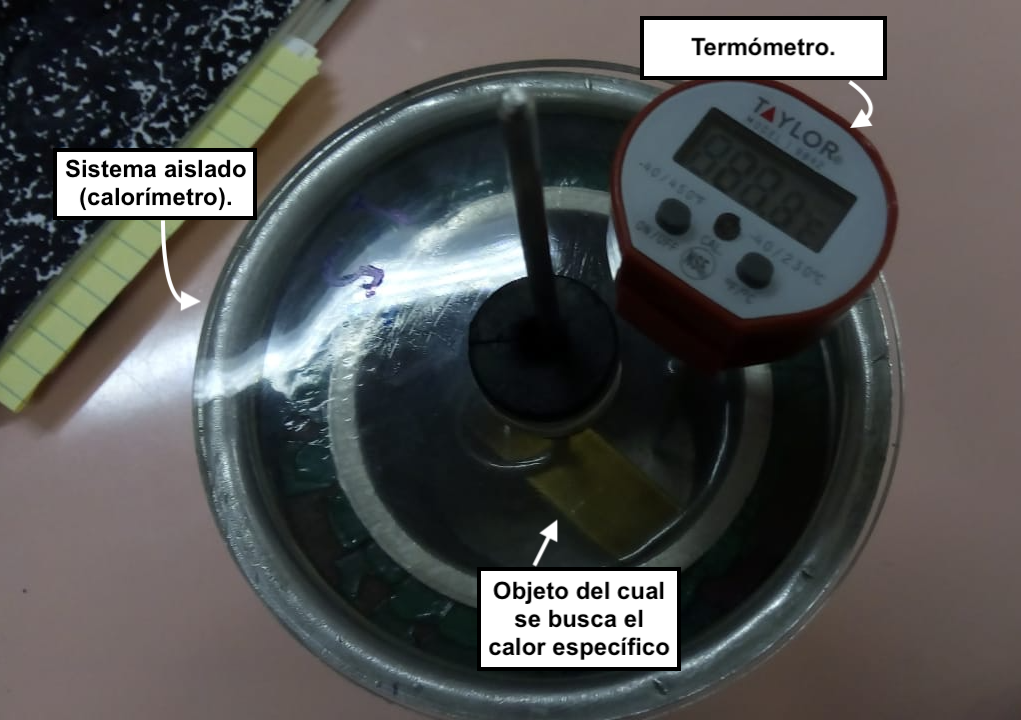
\includegraphics[width=9cm]{Calorimetro.png}
    \caption{Sistema aislado utilizado para las mediciones de temperaturas de equilibrio.}
\end{figure}

Para poder medir la temperatura de equilibrio ($T_{f}$) se esperó un par de minutos después de cerrar el sistema y se usó el agitador para homogeneizar la temperatura. Se midió dicha temperatura ($T_{f}$) y una vez  obtenidas las medidas necesarias y utilizando la conservación de la energía junto con las ecuaciones de calor, se obtiene la ecuación 1.

\begin{equation}\label{ec.2}
    c_{obj}=-\frac{[(m_{H2O}*c_{H20})+(m_{Al}* c_{Al})]* \Delta T_{sis}}{m_{obj}* \Delta T_{obj}}
\end{equation}

Para poder otorgarles incertidumbre a los resultados primero se le atribuyó a las masas: la incertidumbre debida al objeto de medición para la masa del vaso y el objeto metálico que fue de $0.05 gr$, para la masa de agua el doble debido a que es resultado de la diferencia de dos magnitudes con la misma incertidumbre ($1gr$). En cuanto a los calores específicos del agua y el aluminio se consideraron constantes por lo que no se les asocia una incertidumbre en estas consideraciones y para la diferencia de temperatura se utilizó la mínima resolución debido a que proviene de una resta de dos cantidades ($0.1 = 2(0.05)$ºC). Por último, para el promedio de las tres mediciones se le otorgó la máxima diferencia entre valores debido a que se espera que entre más resultados se obtengan de una misma medición, tiendan al mismo valor de manera que otorgar la diferencia más grande aseguramos que esté entre esos valores.

$$\partial c_{obj} = \left|\frac{c_{H20}*\Delta T_{sis}}{m_{obj} * \Delta T_{obj}} \right|dm_{H20} + \left|\frac{c_{Al}*\Delta T_{sis}}{m_{obj} * \Delta T_{obj}} \right|dm_{Al}$$
$$+\left| \frac{(m_{H2O}*c_{H20})+(m_{Al}* c_{Al})}{m_{obj}* \Delta T_{obj}}\right|d\Delta T_{sis}$$
$$+ \left| \frac{[(m_{H2O}*c_{H20})+(m_{Al}* c_{Al})]* \Delta T_{sis}}{m^2_{obj}* \Delta T_{obj}}\right|dm_{obj}$$
$$+ \left|  \frac{[(m_{H2O}*c_{H20})+(m_{Al}* c_{Al})]* \Delta T_{sis}}{m_{obj}* \Delta T^2_{obj}} \right|d\Delta T_{obj}$$


\section*{Resultados.}
Las masas de cada objeto invariante en el experimento fueron:
\begin{itemize}
    \item Masa del vaso del calorímetro: $(49.40\pm0.05)gr $
    \item Masa de objeto plateado: $(59.20\pm0.05)gr $
    \item Masa del objeto dorado: $(182.60\pm0.05)gr $
    \item Masa del objeto cobrizo: $(60.70\pm0.05)gr $
\end{itemize}

Para cada medición se registraron sus valores iniciales de cada apartado y se reportan en la siguiente tabla:
\begin{table}[H]
\begin{center}
\begin{tabular}{|ccc|c|c|c|c|} \hline
  & Color  &  & $m_{H2O}$ [gr] & $T_{cal}$ [ºC] & $T_{obj}$ [ºC] & $T_f$ [ºC] \\
    \hline
    \multicolumn{3}{|c|}{\multirow{3}{*}{Plata}} & $(209.6\pm0.1)$ & $(22.10\pm0.05)$ & $(64.00\pm0.05)$ & $(25.20\pm0.05)$\\ \cline{4-7}
    \multicolumn{3}{|c|}{}& $(209.6\pm0.1) $ & $(24.90\pm0.05)$ &  $(64.00\pm0.05)$ & $(27.60\pm0.05)$ \\ \cline{4-7}
    \multicolumn{3}{|c|}{}& $(233.6\pm0.1)$ & $(23.70\pm0.05)$ & $(75.00\pm0.05)$ & $(26.50\pm0.05)$\\
    \hline
    \multicolumn{3}{|c|}{\multirow{3}{*}{Oro}}& $(145.00\pm0.1)$ & $(27.80\pm0.05)$ & $(54.70\pm0.05)$ & $(30.60\pm0.05)$\\ \cline{4-7}
    \multicolumn{3}{|c|}{}& $(238.50\pm0.1)$ & $(23.30\pm0.05)$ & $(70.00\pm0.05)$ & $(27.20\pm0.05)$\\ \cline{4-7}
    \multicolumn{3}{|c|}{}& $(237.30\pm0.1)$ & $(27.00\pm0.05)$ & $(64.70\pm0.05)$ & $(30.00\pm0.05)$\\
    \hline
    \multicolumn{3}{|c|}{\multirow{3}{*}{Cobre}}& $(206.4\pm0.1)$ & $(26.90\pm0.05)$ & $(60.00\pm0.05)$ & $(28.20\pm0.05)$\\ \cline{4-7}
    \multicolumn{3}{|c|}{}& $(234.4\pm0.1)$ & $(22.20\pm0.05)$ & $(72.30\pm0.05)$ & $(23.60\pm0.05)$\\ \cline{4-7}
    \multicolumn{3}{|c|}{}& $(239.3\pm0.1)$ & $(23.00\pm0.05)$ & $(75.00\pm0.05)$ & $(23.30\pm0.05)$\\
    \hline
\end{tabular}
\end{center}
\label{tab:multicol}
\caption{Datos obtenidos de los metales, se realizaron 3 mediciones por metal. Donde: $m_{H2O}$ es masa del agua, $T_{cal}$ es la temperatura del calorímetro, $T_{obj}$ es la temperatura a la cual se introdujo el metal y $T_f$ la temperatura de equilibrio.}
\end{table}

Utilizando la ecuación 1 se obtienen los siguientes resultados:

\begin{table}[H]
    \centering
    \begin{tabular}{ |c|c|c|c| } 
\hline
Color & Calor específico ($\frac{cal}{gr{\circ}C}$) & $C_e$ promedio ($\frac{cal}{gr{\circ}C}$) \\
\hline

\multirow{3}{4em}{Plata} & $0.297 \pm 0.011$ &  \\ 
& $0.276 \pm 0.011$ & $0.27 \pm 0.03$ \\ 
& $0.238 \pm 0.009$ &  \\ 
\hline

\multirow{3}{4em}{Oro} & $0.099 \pm 0.013$ &  \\ 
& $0.124 \pm 0.011$ & $0.113 \pm 0.014$ \\ 
& $0.117 \pm 0.014$ &  \\ 
\hline

\multirow{3}{4em}{Cobre} & $0.146 \pm 0.012$ &  \\ 
& $0.116 \pm 0.009$ & $0.10 \pm 0.09$ \\ 
& $0.024 \pm 0.008$ &  \\ 
\hline

\end{tabular}
    \caption{Calores específicos asociados a los datos de Tabla 1 y calor específico promedio de cada material.}
    \label{Tabla 2}
\end{table}





\section*{Conclusiones.}

En cuanto a calores específicos, el del objeto plateado resultó ser mayor que los otros dos, sin embargo el más exacto fue el de color oro ya que todas las mediciones tienen un rango de intersección. En cuanto a la segunda cifra significativa, la incertidumbre en todos es relativamente grande; aún así podemos asegurar que en los objetos dorado y plateado, la primera cifra significativa es 0.1 y 0.2 respectivamente. En cuanto al tercer objeto, el de color cobrizo, sus resultados difieren demasiado entre ellos, para garantizar certeza al calor específico es necesario hacer mas veces el experimento con este objeto.

Si seleccionamos los datos que parecen ser más cercanos al valor real del tercer objeto, es decir tomamos en cuenta los dos primeros, el $C_{cobre} = 0.131 \pm 0.015$ que de hecho equidista de ambas mediciones, no obstante, es por la tercera medida, por la cual se cree es necesario realizar nuevas mediciones ya que probablemente se cometió un error en la medición. Para mejorar el resultado se propone una medición donde se obtenga una temperatura más confiable en cuanto al objeto utilizado, debido a que se utilizó un método en el cual se medía fuera del agua que lo calentó, se propone no separar estos dos sistemas (el objeto a calentar y el agua) y medir la temperatura de estos en equilibrio.

Por último, si se buscan metales los cuales tienen calores específicos cercanos a los que se obtuvieron se observa que el calor específico del objeto plateado es un valor cercano al del aluminio ($C_{al} = 0.215 \frac{cal}{gr{\circ}C}$), el de color oro al del latón ($C_{la} = 0.094 \frac{cal}{gr{\circ}C}$) y el acero ($C_{ac} = 0.106 \frac{cal}{gr{\circ}C}$). El tercero tiene una incertidumbre del 90\% que lo vuelve inútil para comparación pues muchos metales entran en el intervalo que arrojan las mediciones.

\section{Bibliografía.}

    Oda, B.,  Universidad Nacional Autónoma de México. Facultad de Ciencias. (2005). Introduccion al analisis grafico de datos experimentales (3ª ed.). Ciudad de México, México: UNAM, Facultad de Ciencias.
    
    Serway, R. A.,  Jewett, J. W. (2016). Física para Ciencias e Ingeniería Vol.1 (9ª ed.). Ciudad de México, México: Cengage Learning.
    


\end{document}



